  
\documentclass[letterpaper, 12 pt]{article}
\usepackage{indentfirst}
\usepackage{color}
\usepackage{hyperref}
\usepackage{graphicx}
\usepackage[portuguese]{babel}
\hypersetup{
    colorlinks,
    linktoc=all,
    citecolor=black,
    filecolor=black,
    linkcolor=black,
    urlcolor=black
}


\renewcommand{\contentsname}{Sumário}

% -------------------------------------------------------------------------------------
% BEGIN DOCUMENT
% -------------------------------------------------------------------------------------
\begin{document}
\title{Manual de Utilização do Sistema de Controle de Estoque Bloco K}
\author{Departamento de Tecnologia da Informação - CECRF}
\maketitle
\pagestyle{empty}
\newpage


% -------------------------------------------------------------------------------------
% TABLE OF CONTENTS
% -------------------------------------------------------------------------------------
\tableofcontents
\newpage

% -------------------------------------------------------------------------------------
% INTRODUCTION
% -------------------------------------------------------------------------------------
\section{Introdução}
Sistema desenvolvido para controlar e rastrear os insumos recebidos pelo Centro de Radiofarmácia.
\newpage


\section{Acesso ao sistema}
Para seu desenvolvimento, foi utilizado como navegador padrão o Google Chrome, mas o software pode ser utilizado 
no Mozila Firefox e Microsoft Edge. Preferencialmente a indicação é o navegador do Google.
\subsection{URL de acesso}
Digite no navegador o seguinte endereço: http://10.0.4.7:8080/www
\subsection{Login}
A seguinte página, Fig. \ref{figura:login1}, deve abrir após o acesso pela URL. Uma vez logado, o sistema grava num token as credenciais (email e senha), onde fica armazenado por 24 horas, sendo desnecessário novo login neste espaço de tempo.
O novo usuário deve se cadastrar clicando no botão registrar.  

\begin{figure}[h]
\centering % centralizar figura
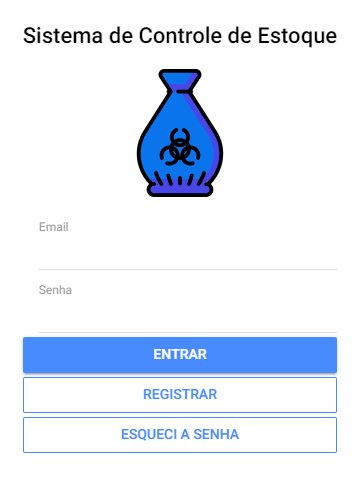
\includegraphics[width=5cm]{imagens/login1.PNG}
\caption{Tela inicial de login}
\label{figura:login1}
\end{figure}
\newpage

\subsection{Registrar - Novo Usuário}
Na  Fig. \ref{figura:registrar1} temos o formulário de cadastro de um novo usuário. Os camopos com asterisco são obrigatórios, e o email inserido deve ser válido e será utilizado como login de acesso. 

\begin{figure}[h]
\centering % centralizar figura
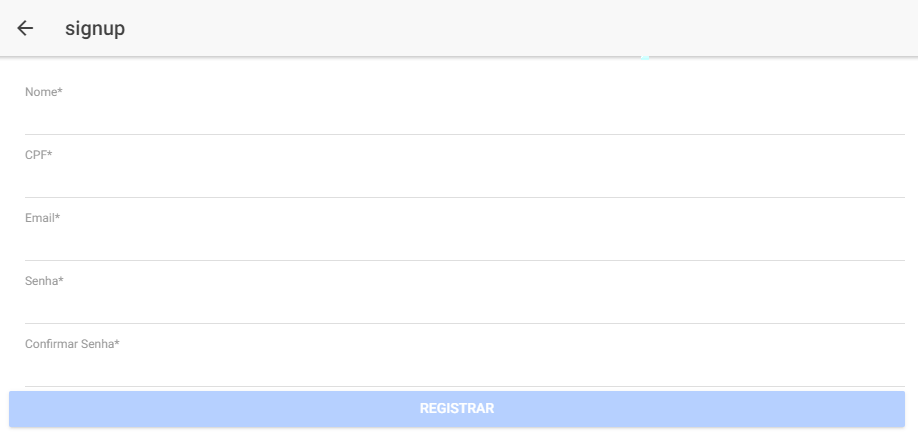
\includegraphics[width=10cm]{imagens/registrar1.PNG}
\caption{Registro de novo usuário}
\label{figura:registrar1}
\end{figure}

\section{Software}
Após logado, o sistema redireciona para a tela principal, Fig. \ref{figura:dashboard1}, identificada como Dashboard, trazendo informações relevantes sobre o estado atual de insumos no banco de dados. Ao lado do nome Dashboard podemos acessar o menu onde contem todos os links para as páginas do sistema, Fig. \ref{figura:menu1}.

\begin{figure}[h]
\centering % centralizar figura
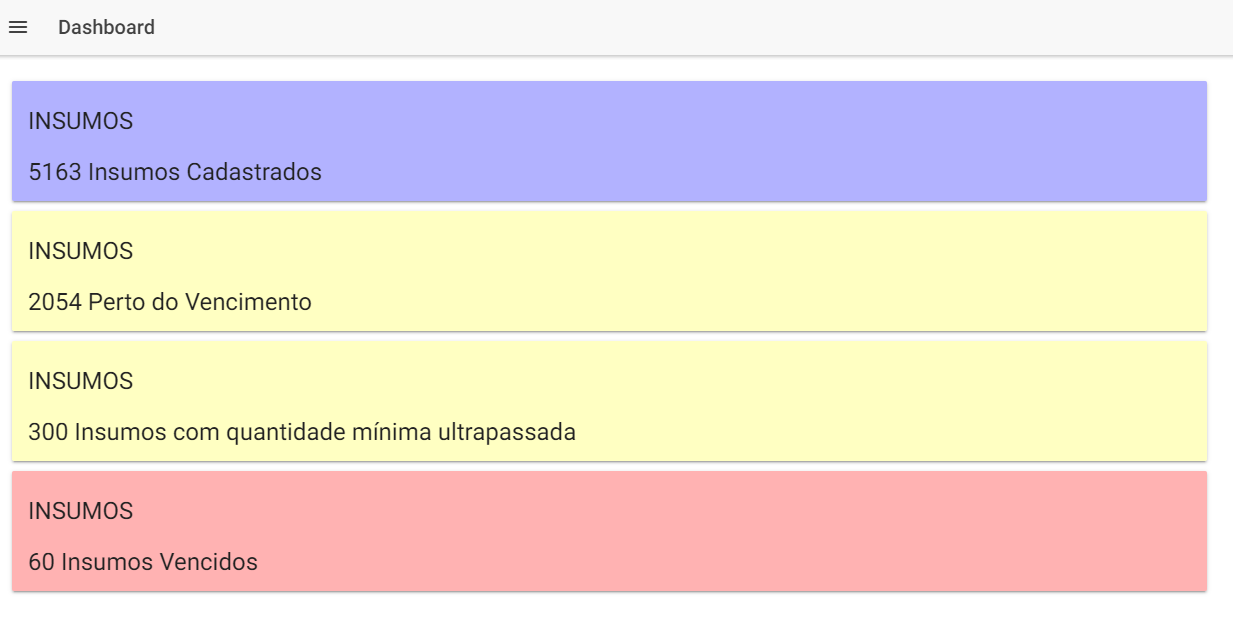
\includegraphics[width=9cm, height=4cm]{imagens/dashboard1.PNG} 
\caption{Tela inicial do software}
\label{figura:dashboard1}
\end{figure}

\subsection{Menu do Software}
Neste momento, podemos acessar todas as páginas do software. Abaixo uma breve descrição de cada link:

\begin{itemize}
  \item Dashboard:
  \item Produção:
  \item Insumos:
  \item Produtos:
  \item Categorias:
  \item Fornecedores:
  \item Unidades de Medida:
  \item Localizações:
  \item Movimentações:
  \item Entradas:
  \item Saídas:
  \item Profile:
  \item Logout:
\end{itemize}

\begin{figure}[h]
\centering % centralizar figura
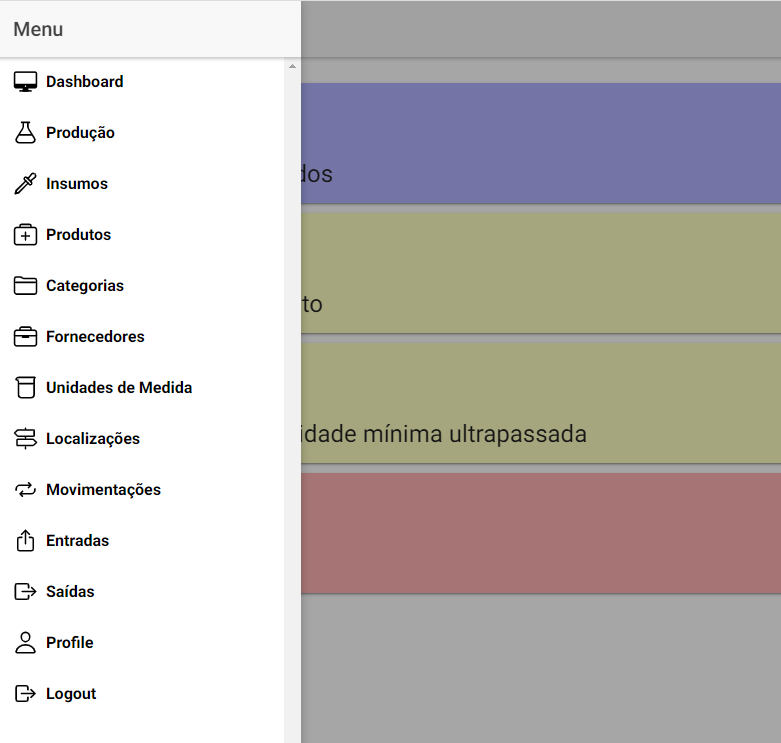
\includegraphics[height=4cm]{imagens/menu1.PNG} 
\caption{Tela inicial do software}
\label{figura:menu1}
\end{figure}
% -------------------------------------------------------------------------------------
% REFERENCES
% -------------------------------------------------------------------------------------
%\bibliography{}

% -------------------------------------------------------------------------------------
% END DOCUMENT
% -------------------------------------------------------------------------------------
\end{document}